\chapter{Marco Teórico}
\section{Leyes Fundamentales}
En esta sección se desarrollarán las ecuaciones que rigen el movimiento de los fluidos, tomando como base, las leyes fundamentales de conservación para un elemento diferencial.
\subsection{Mecánica de Fluidos}
Primero, se generalizarán las ecuaciones, a modo de tener un marco lo suficientemente amplio para después aplicarlo específicamente a la dinámica atmosférica y así extraer las ecuaciones primitivas de la atmósfera.
\subsubsection{Conservación de la Masa}
La conservación de la masa queda descrita en el sentido euleriano de la forma:
\begin{equation}
\partial_t \rho + \partial_i(\rho u_i) = 0
\end{equation}
donde el primer término corresponde a la acumulación de masa dentro de un elemento diferencial de fluido, y el segundo, a los flujos de masa por las fronteras.

Aunque la atmósfera es un fluido que a grandes rasgos es compresible, es válido hacer la aproximación de incompresibilidad debido a que los movimientos de las masas de aire rara vez exceden el $\text{Ma }=0.3$. Para el caso incompresible se tiene entonces:
\begin{eqnarray}
\rho = \rho_0 = \text{cte.} \\
\partial_i u_i =0
\end{eqnarray}

Implicando que el volumen de un elemento diferencial de fluido se mantiene constante en toda su trayectoria material.
\subsubsection{Conservación de la Cantidad de Movimiento}
ley de newton en forma general, fuerzas de superficie y de cuerpo, describir cada fuerza, órdenes de magnitud, aproximaciones.
\subsubsection{Conservación de la Energía}
energía cinética, energia térmica.
\subsection{Dinámica Atmosférica}
a través de las ecuaciones anteriores deducir las ecuaciones primitivas, introducir temperatura potencial, geopotencial y otra def atmofericas
\subsection{Teoría de la Capa Límite Atmosférica}
Se define la capa límite atmosférica (ABL) como la parte de la troposfera que está influenciada directamente por la presencia de la superficie terrestre y responde a las fuerzas superficiales en una escala de tiempo del orden de las horas o menor.

explicar fenomenos de la abl, turbulencia, explicar transporte turbulento e introducir la descomposición de Reynolds.
\section{Turbulencia Hidrodinámica}
\subsection{Fundamentos}
naturaleza de la turbulencia, fenomenología, 
\subsection{Cascada de Energía}
hipótesis de kolmogorov, derivar ley -5/3, espectro de energía cinética turbulenta.
\subsection{Hipótesis de Taylor}
Debido a la dificultad operativa y numérica que presenta el tener información instantánea de un campo de flujo en la capa límite atmosférica para caracterizar los distintos tamaños de los vórtices, G.I. Taylor sugirió que para ciertos casos especiales, es posible obtener información acerca del espectro de energía solo utilizando mediciones en un solo punto del espacio sobre un periodo de tiempo prolongado.

En la simplificación de Taylor, se habla de turbulencia congelada, es decir, el tiempo característico asociado a los vórtices turbulentos es muy menor que el tiempo característico de advección de los mismos.

Sea $\phi$ una variable cualquiera, la hipótesis queda expresada como:
\begin{equation}
D_t\phi = 0
\end{equation}

Entonces, al desarrollar la derivada material, la forma general de la hipótesis de turbulencia congelada de Taylor es de la forma:
\begin{equation}
\partial_t \phi = -u_i\partial_i \phi
\end{equation}

Para los fenómenos dentro de ABL, los cuales son predominantemente horizontales, es conveniente dejar todo expresado en función de la rapidez horizontal del viento $V_h =\sqrt{u^2+v^2}$. De esta forma se tiene:
\begin{equation}
\partial_t \phi = -V_h\partial_{x_h}\phi
\end{equation}
donde $x_h$ es la dirección horizontal del viento.

Expresada en términos de la frecuencia y número de onda:
\begin{equation}
\kappa = \frac{f}{V_h}
\end{equation}

Finalmente, la condición de turbulencia congelada es válida para un punto fijo según la sugerencia de Willis y Deardorff (1976):
\begin{equation}
\sigma_{V_h}<0.5\cdot V_h
\end{equation}
donde $\sigma_{V_h}$ es la desviación estándar de la velocidad horizontal del viento. Este valor es una medida de la intensidad de la turbulencia. Es decir, la hipótesis de Taylor se debe cumplir para flujos en donde la intensidad de la turbulencia de pequeña en relación a la rapidez del flujo medio.
\section{Large Eddy Simulation}
Considerando entonces la naturaleza multiescala de la turbulencia, es natural querer resolver los campos de flujo separando las escalas de producción (relacionadas con los grandes vórtices y el ingreso de energía) de las microescalas (relacionadas a los vórtices en la escala de Kolmogorov y a la disipación de energía). 

La manera de realizar esto es aplicando un filtro a las variables de modo que actúe al nivel del espectro de energía, separando las escalas grandes de las pequeñas. Se introduce entonces el operador de filtrado según Leonard(1974).
\begin{equation}
\overline{\phi}(x_i,t) = \int G(r_i,x_j)\phi(x_j-r_i,t)dr_i
\end{equation}
Donde la integración se realiza en todo el dominio del flujo. Notar que el filtro corresponde a una operación de convolución en el sentido del análisis de Fourier. El kernel $G$ del filtro satisface una condición de normalización:
\begin{equation}
\int G(r_j,x_i)dr_j = 1
\end{equation}
Se define entonces una magnitud residual basada en la operación de filtrado como:
\begin{equation}
\phi' = \phi - \overline{\phi}
\end{equation}
Es decir, se depara la variable de interés en una parte filtrada y su residuo. Está descomposición es, a priori, análoga a una descomposición de Reynolds.

Se debe tener en cuenta que el filtro es en el fondo un nuevo operador matemático que cumple sus propias propiedades y que permite separar las escalas grandes de las pequeñas. Para una mejor descripción teórica de lo que implica un operador de filtrado se puede recurrir a las referencias...

falta mucho...

\section{Data Assimilation}

\section{Simulación Numérica Multiescala}
Tal como se describió en la anteriormente, el comportamiento de un fluido está sujeto a la acción de diversos actores que son los miembros que componen las ecuaciones fundamentales. En el caso de una simulación multiescala, la predominancia de los términos dentro de las ecuaciones no es única, es decir, en una escala donde la longitud característica sea del orden de los 100 [km], las fuerzas asociadas a la rotación de la tierra son de primer orden y en cambio las fuerzas viscosas pueden ser válidamente despreciadas, sin embargo, en una escala donde la longitud característica sea del orden de 1 [m], la importancia de la viscosidad no se puede despreciar y también es necesario comenzar a incorporar otros mecanismos como puede ser la flotación y la turbulencia.

Este problema dentro de la simulación, separa las áreas del conocimiento y de la aplicación de la mecánica de los fluidos, tal como se puede apreciar en la figura \ref{fig:escalas}

\begin{figure}[H]
\centering
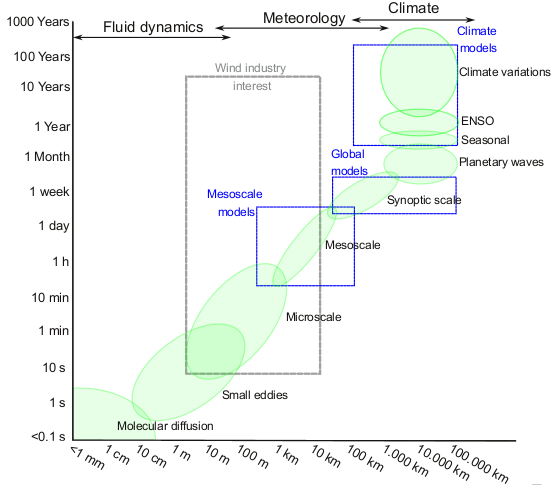
\includegraphics[width=0.7\linewidth]{Imagenes/terraincog}
\caption{Separación de escalas en simulación de mecánica de fluidos.}
\label{fig:escalas}
\end{figure}

Cuando se lleva este problema a la modelación de la turbulencia, aparece un fenómeno especial denominado \emph{Terra Incognita}.

Utilizando la terminología de Wyngaard (2004), sea $\Delta$ la escala del filtro espacial asociado a la solución de las ecuaciones de movimiento y $l$ la escala característica de los vórtices en el rango inercial. La Figura \ref{fig:terra} muestra como se vería el espectro de energía turbulenta dentro de estas escalas.
\begin{figure}[H]
	\centering
	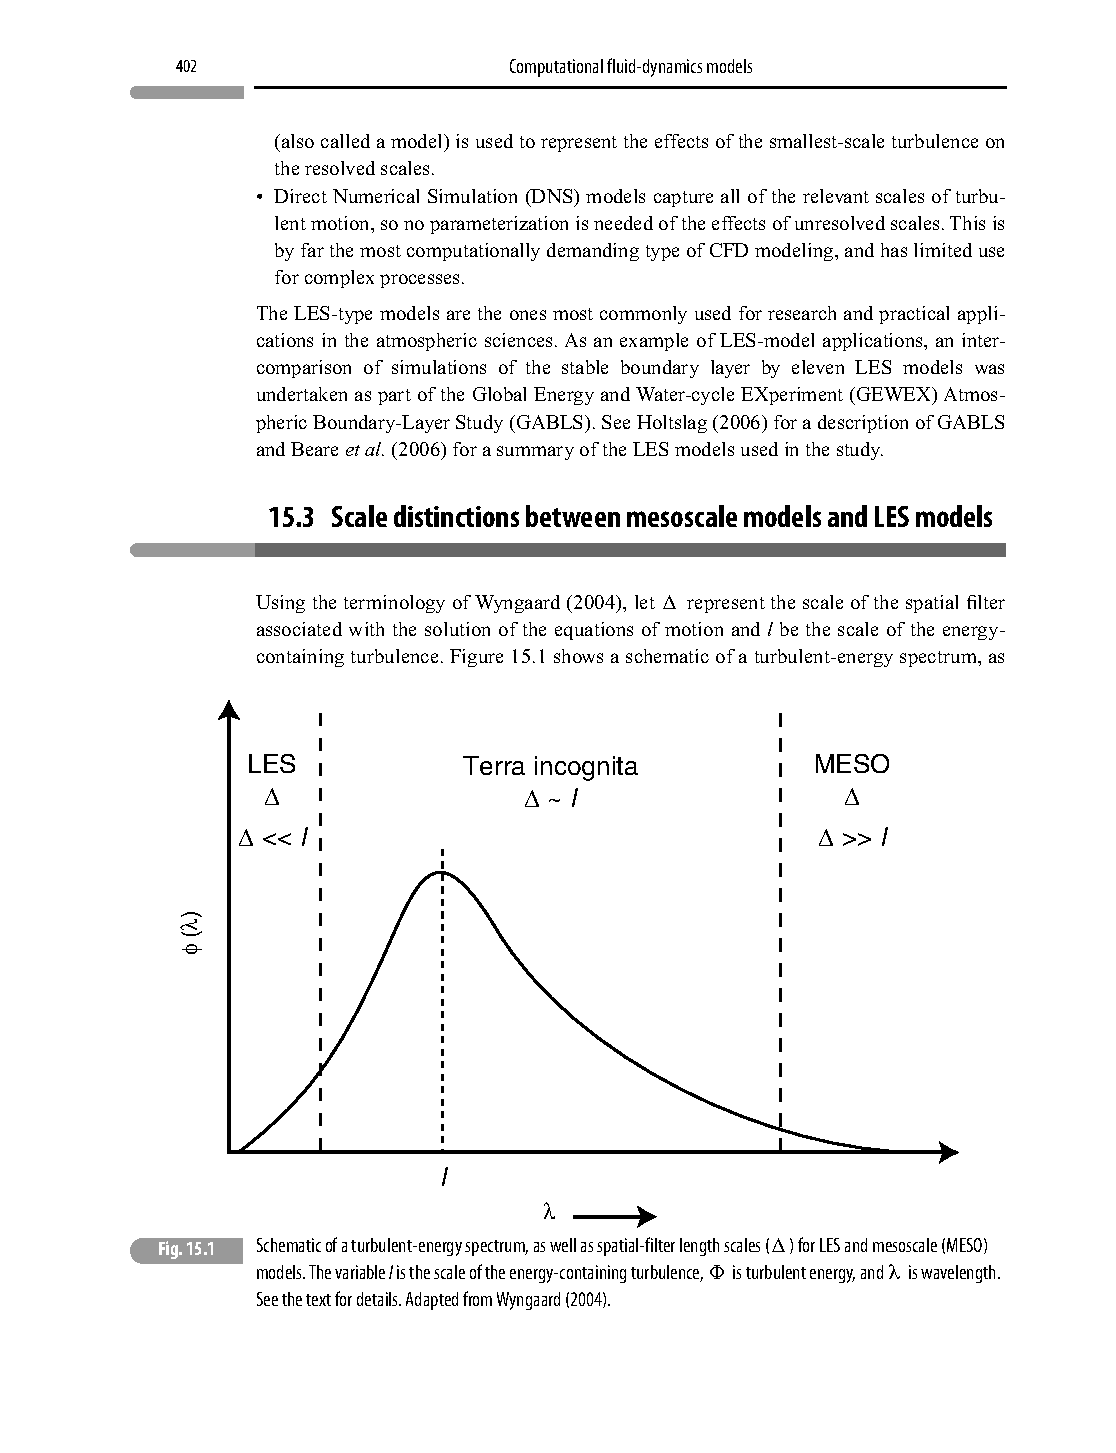
\includegraphics[width=0.8\linewidth,trim={2cm 3cm 2cm 11.5cm},clip]{Imagenes/terra}
	\caption{Espectro de energía turbulenta multiescala.}
	\label{fig:terra}
\end{figure}

Para valores de $\Delta\gg l$ asociados a la mesoescala, la producción de energía turbulenta queda por debajo del filtro y por lo tanto, tiene sentido que se modele a través de un esquema de submalla. Por otro lado, para valores de $\Delta\ll l$ los vórtices que contienen la energía pueden ser completamente modelado por las ecuaciones y entonces no debe usarse un SGS (microescala).

Queda entonces el rango en donde $\Delta\sim l$. Dentro de este intervalo se desconoce cual es el comportamiento de los modelos atmosféricos ya que existe una doble representación de tanto los vórtices que se resuelven como los que se modelan.

En la práctica, el acercamiento para compensar este problema es definir los dominios de modo que se evite usar el modelo en el rango de la \emph{Terra Incognita}.
\section{ARW-WRF}
\subsection{Generalidades}
El modelo ARW-WRF (Advanced Research WRF) es un modelo no hidrostático que resuelve el sistema de ecuaciones para flujo compresible en su forma conservativa y utilizando una coordenada vertical de masa (o de presión hidrostática). Su coordenada vertical está definida como:
\begin{equation}
\eta = \frac{p_{dh}-p_{dht}}{\mu_d}
\end{equation}
Donde $p_{dh}$ corresponde a la componente hidrostática de la presión del aire seco, y:
\begin{equation}
\mu_d = p_{dhs} - p_{dht}
\end{equation}
es la masa de aire seco para una columna. En estas ecuaciones los subíndices $t$ y $s$ corresponden a los límites superior (top) e inferior (surface) del dominio. Las variables principales que resuelve el modelo son las velocidades covariantes $(u,v,w)$, masa de aire seco, geopotencial, temperatura potencial ($\theta$) y energía cinética turbulenta (TKE) de submalla (SGS). La ecuación de momentum, temperatura potencial, SGS TKE y otros escalares relevantes tienen una forma acoplada con la masa de aire seco, a priori:
\begin{equation}
\partial_t (\mu_d\theta) + \partial_x(\mu_d u \theta)+\partial_y(\mu_d v \theta)+\partial_\eta (\mu_d \omega \theta) = F
\end{equation}
Donde $F$ es la suma de la mezcla turbulenta junto con otras fuerzas y
\begin{equation}
\omega = d_t\eta
\end{equation}
es la velocidad en la coordenada vertical.

La discretización en el tiempo se realiza a través de un esquema de integración temporal múltiple. Este esquema separa los modos de alta frecuencia (i.e. ondas acústicas y de gravedad) de los modos de baja frecuencia (modo físico). ARW utiliza un esquema RK3 y durante cada paso en el RK, el modo de alta frecuencia que se propaga horizontalmente es integrado a través de un esquema \emph{forward-backward} utilizando un paso de tiempo acústico, que es típicamente un orden de magnitud mas pequeño que el paso físico, mientras que un esquema implícito es utilizado para el modo de alta frecuencia que se propaga de manera vertical.
\subsection{Ecuaciones Resueltas}
ecuaciones de euler, derivacion de las ecuaciones completas, etc.
\subsection{Discretización Espacial}
malla vertical, malla horizontal, arakawa c-grid, metodos anidados
\subsection{Discretización Temporal}
pasos de tiempo físico y acustico, pasos del rk3
\subsection{Aspectos Numéricos}
\subsubsection{Filtros}
filtro acustico, filtro polar, otros filtros
\subsubsection{Advección}
discretizacion numerica de la adveccion, limitadores, etc.
\subsubsection{Difusión}
La difusión y los flujos turbulentos calculados según el espacio físico $(x,y,z)$ se calculan haciendo uso de la métrica del espacio:
\begin{eqnarray}
z_x=g^{-1}\delta_x\phi \\
z_y=g^{-1}\delta_y\phi
\end{eqnarray}

El término difusivo se agrega al lado derecho de las ecuaciones de Euler, junto al resto de las fuerzas externas. Estas se ven:
\begin{eqnarray}
\partial_t U = \ldots - m_x[\partial_x\tau_{11}+\partial_y\tau_{12}-\partial_z(z_x\tau_{11}+z_y\tau_{12})]-\partial_z\tau_{13} \\
\partial_t V = \ldots - m_y[\partial_x\tau_{12}+\partial_y\tau_{22}-\partial_z(z_x\tau_{12}+z_y\tau_{22})]-\partial_z\tau_{23} \\
\partial_t W = \ldots - m_y[\partial_x\tau_{13}+\partial_y\tau_{23}-\partial_z(z_x\tau_{13}+z_y\tau_{23})]-\partial_z\tau_{33}
\end{eqnarray}

Y el tensor de esfuerzos viscosos es:
\begin{equation}
\tau_{ij} = -\mu_d K_{h,v}S_{ij}
\end{equation}
donde $K_{h,v}$ es la viscosidad turbulenta en dirección horizontal o vertical según la ecuación y $S_{ij}$ es el tensor tasa de deformación.

La viscosidad turbulenta se calcula en función de la energía cinética turbulenta $e$ de la forma:
\begin{equation}
K_{h,v}=C_k l_{h,v}\sqrt{e}
\end{equation}
donde $C_k$ es una constante (normalmente $0.15<C_k<0.25$) y $l$ es un largo característico que se calcula en función de la isotropía de la malla, la resolución, $e$ y la estratificación.

La ecuación de transporte para $e$ es:
\begin{equation}
\partial_t(\mu_d e) + (\partial_i V_i e)_\eta = \mu_d(\text{ producción + flotación + disipación})
\end{equation}
falta detallar el resto de la ecuaciones, modelo de smagorinsky.
\subsubsection{Microfísicas}
detallar cada microfísica y su incorporacion a las ecuaciones

\chapter{Caso de Estudio}
\section{Aspectos Generales}
Para este caso, se está interesado en caracterizar el comportamiento del viento en la zona costera de Valparaíso, mas específicamente en el sector de Laguna Verde, lugar donde existe un gran interés a causa de su alto potencial eólico, tal como lo explicita el Explorador Eólico de la Universidad de Chile y cuyo resultado se puede observar en la figura \ref{fig:explorador}.

\begin{figure}[H]
	\centering
	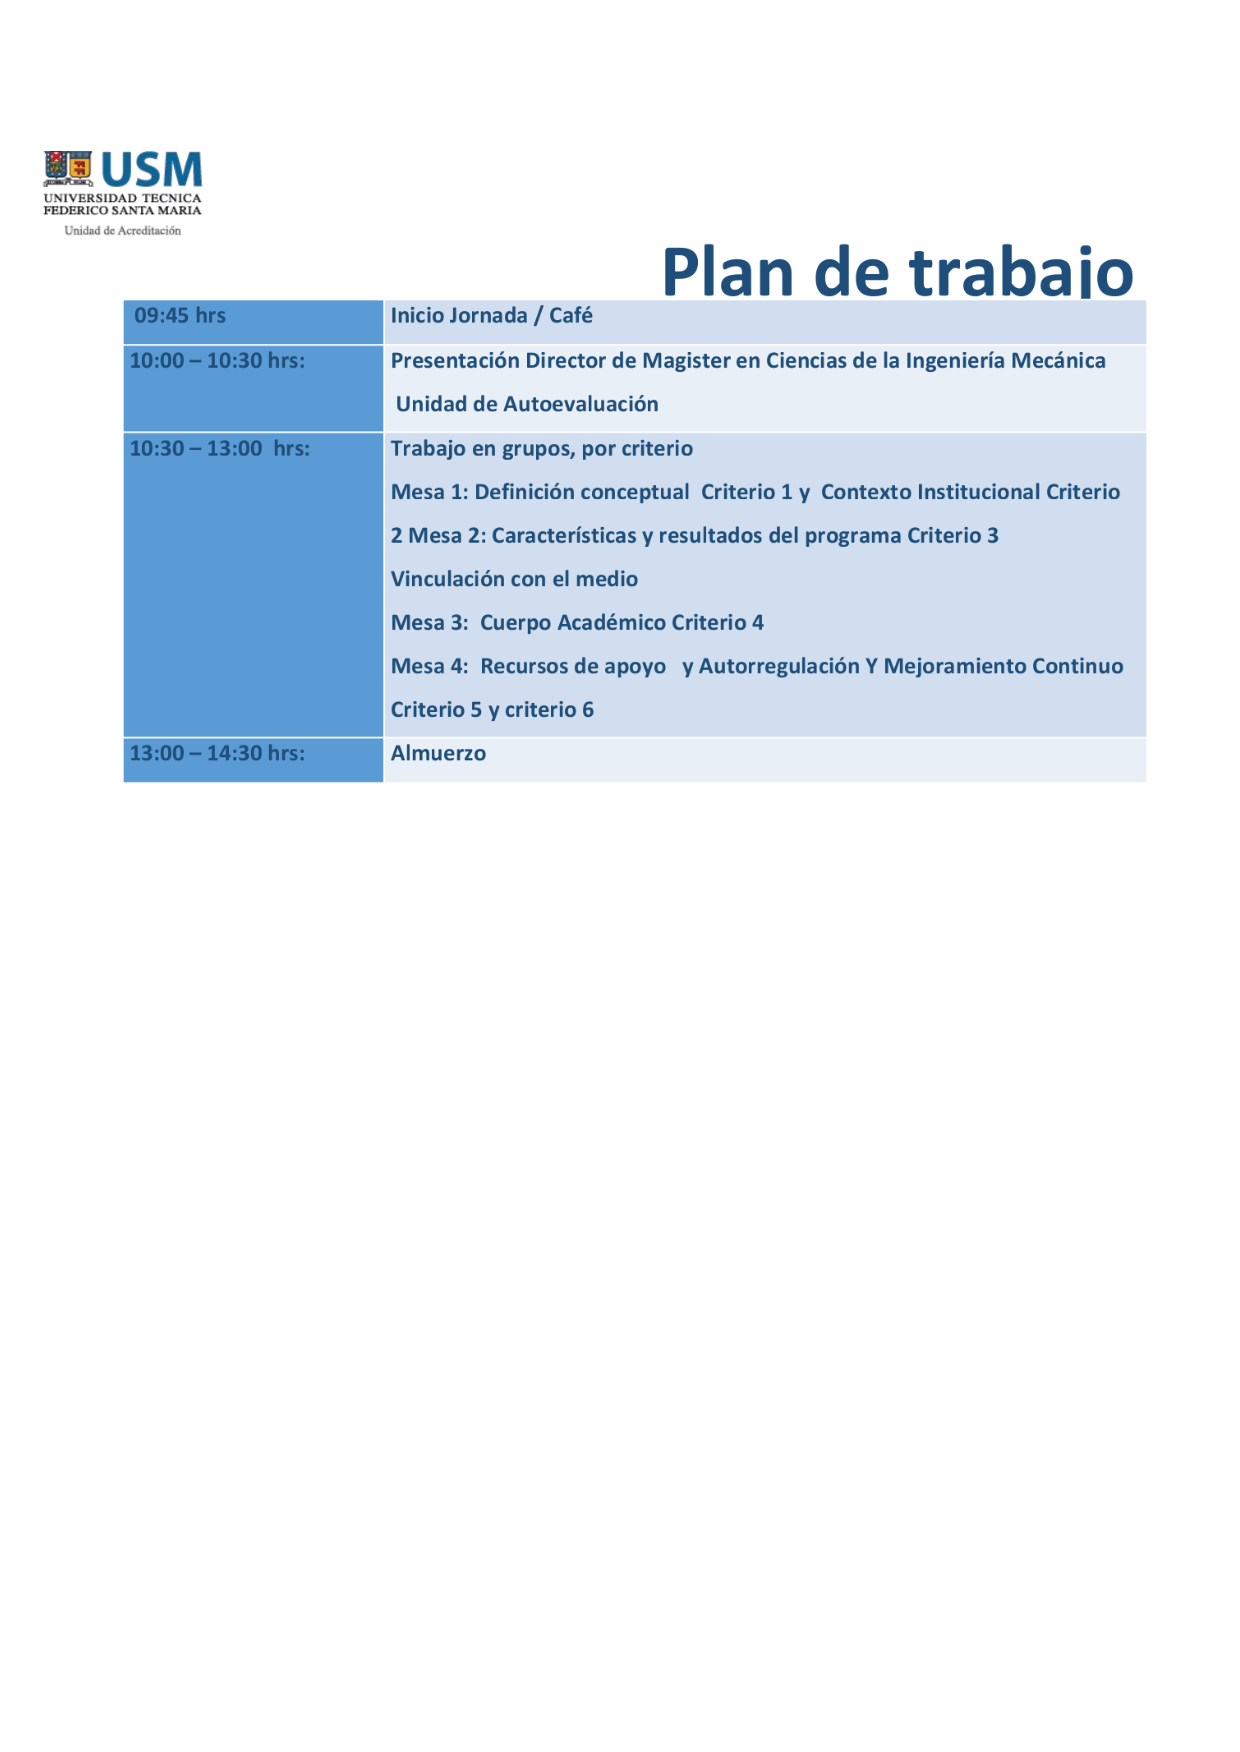
\includegraphics[width=0.9\linewidth,trim={5.4cm 2cm 15cm 5.5cm},clip]{Imagenes/explorador}
	\caption{Información del Explorador Eólico para la zona de interés.}
	\label{fig:explorador}
\end{figure}

Los datos de la figura \ref{fig:explorador} corresponde a un promedio anual para la magnitud de la velocidad en cada punto de la malla numérica. Esta malla tiene una resolución de 1 [km], la cual, si bien permite obtener información relevante acerca de zonas con alto potencial eólico, es ineficiente para capturar el comportamiento del flujo en el terreno complejo. Es por esto, que es relevante afinar la simulaciones aplicando técnicas modernas y apuntar a una mejor calidad para la caracterización eólica de una zona.

La simulación de la que trata este informe se realiza en un día standart del mes de Enero del año 2010. El día de simulación se escogió, por una parte, por las facilidades para obtener las condiciones de contorno provenientes de otros modelos y por otro, por que en verano existe un comportamiento mas energético del viento.

La ventana de viento elegida para simular es de 9:00 a 21:00, horario donde existe una mayor relevancia de los efectos térmicos de la superficie. Si bien la ventana de tiempo es de 12 horas, solo se pueden extraer resultados válidos luego de pasadas las primeras 3 horas de simulación como se verá mas adelante. Por lo tanto la simulación válida corre desde las 12:00 hasta las 21:00.
\section{Resolución Espacial}
Se discretiza espacialmente la zona en 6 dominios colocados de forma telescópica y centrados en el punto de coordenadas (-33.097344, -71730552) que corresponde a la costa de Punta Curaimilla.

Como el objetivo principal es obtener una malla fina con resolución de 50 [m], a la malla mas gruesa se le asigna un $\Delta x = \Delta y = 12150$ [m] y cada malla se va afinando en un factor de 3 su resolución. La resolución de malla mas gruesa es electa debido a su compatibilidad con la interpolación de las condiciones de borde del modelo global.

La distribución de las mallas y su proyección sobre la tierra se pueden observar en las figuras \ref{fig:0102}, \ref{fig:0203}, \ref{fig:0304}, \ref{fig:0405} y \ref{fig:0506}.

\begin{figure}[H]
	\centering
	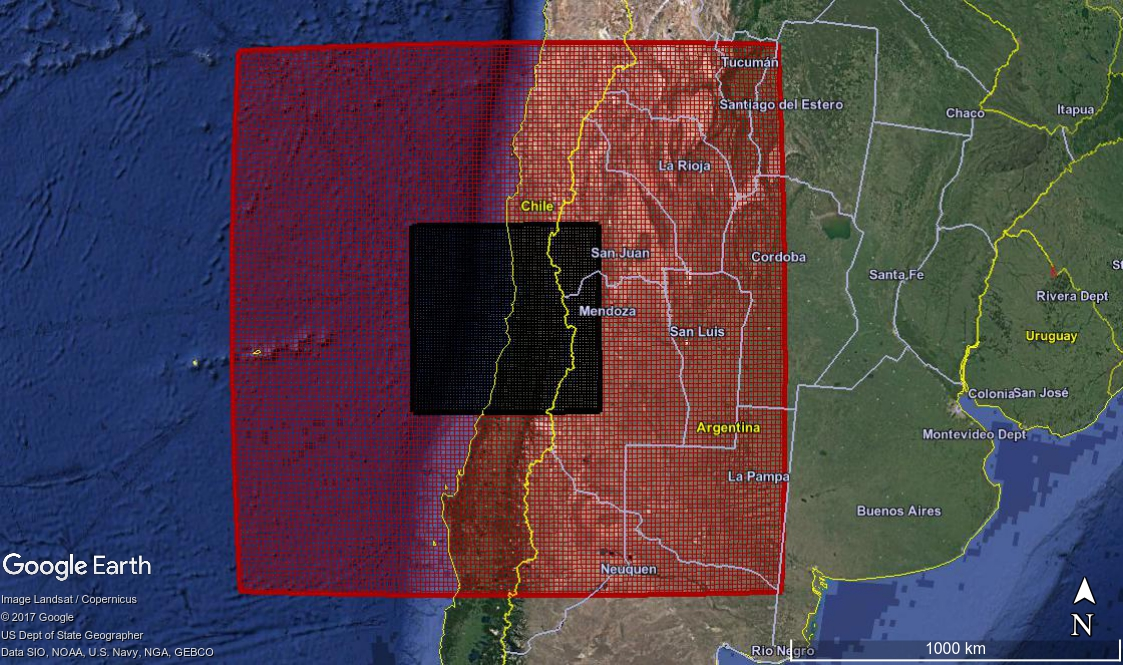
\includegraphics[width=0.95\linewidth]{Imagenes/d06d05}
	\caption{Dominios de las mallas exteriores d01 y d02.}
	\label{fig:0102}
\end{figure}

\begin{figure}[H]
	\centering
	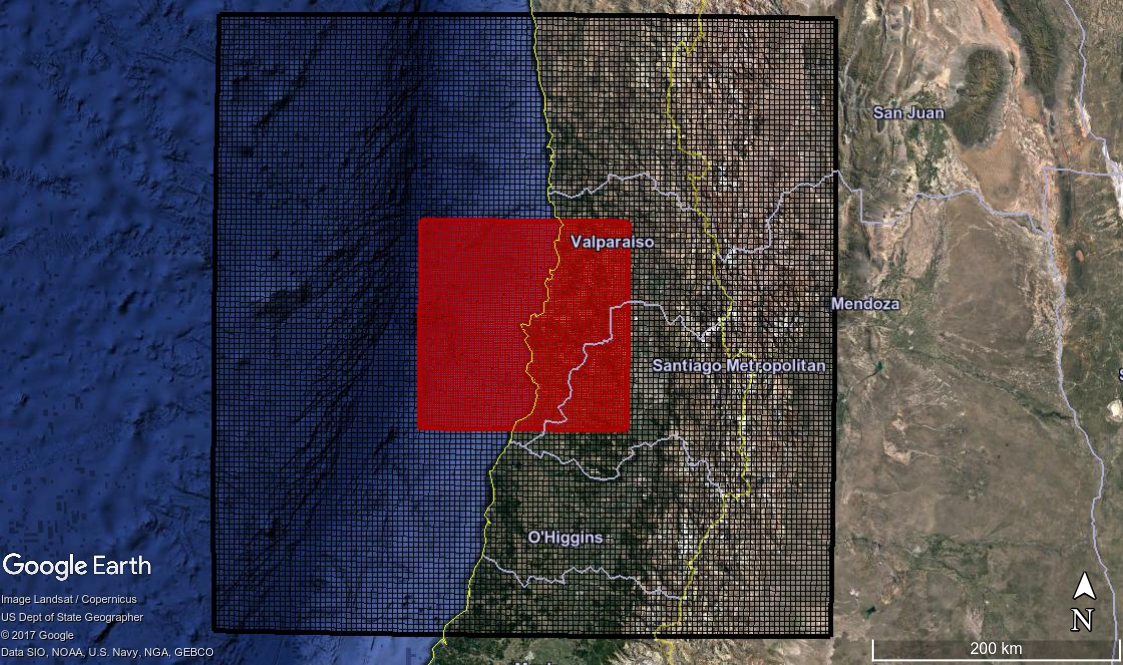
\includegraphics[width=0.95\linewidth]{Imagenes/d05d04}
	\caption{Dominios d02 y d03.}
	\label{fig:0203}
\end{figure}

\begin{figure}[H]
	\centering
	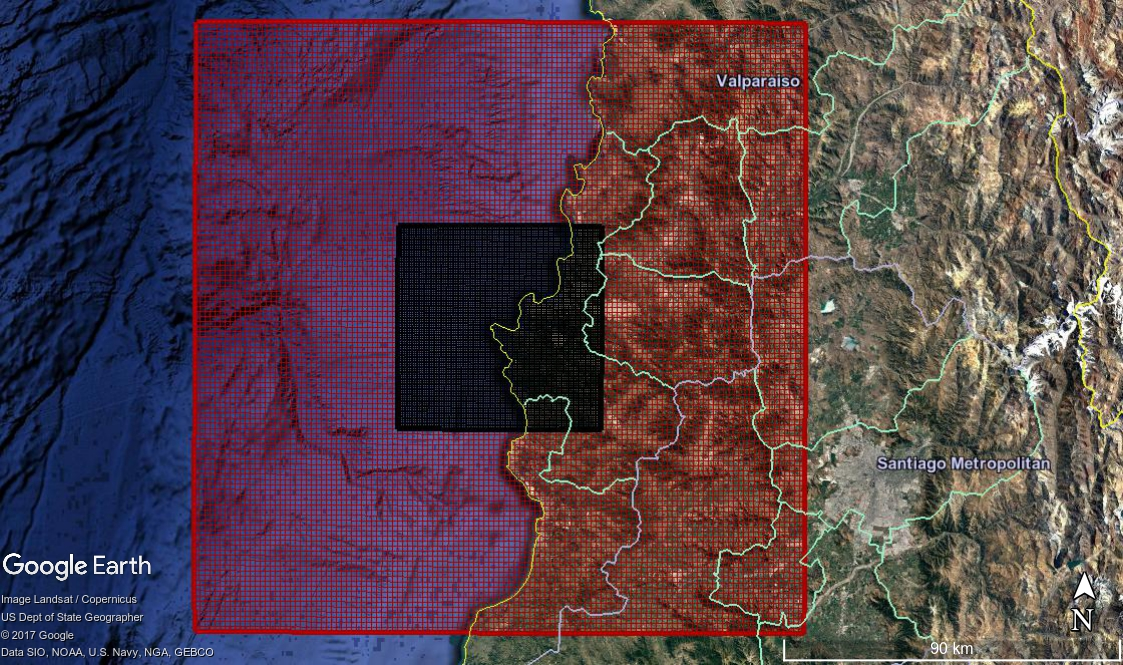
\includegraphics[width=0.95\linewidth]{Imagenes/d04d03}
	\caption{Dominios d03 y d04 (LES).}
	\label{fig:0304}
\end{figure}

\begin{figure}[H]
	\centering
	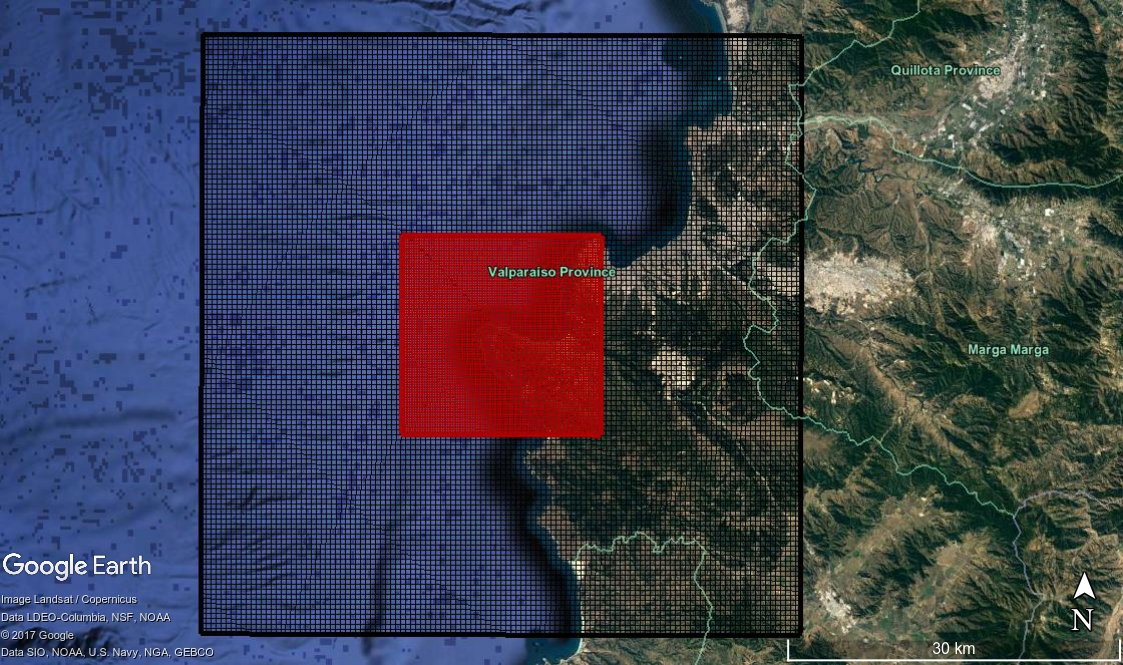
\includegraphics[width=0.95\linewidth]{Imagenes/d03d02}
	\caption{Dominios d04 (LES) y d05 (LES).}
	\label{fig:0405}
\end{figure}

\begin{figure}[H]
	\centering
	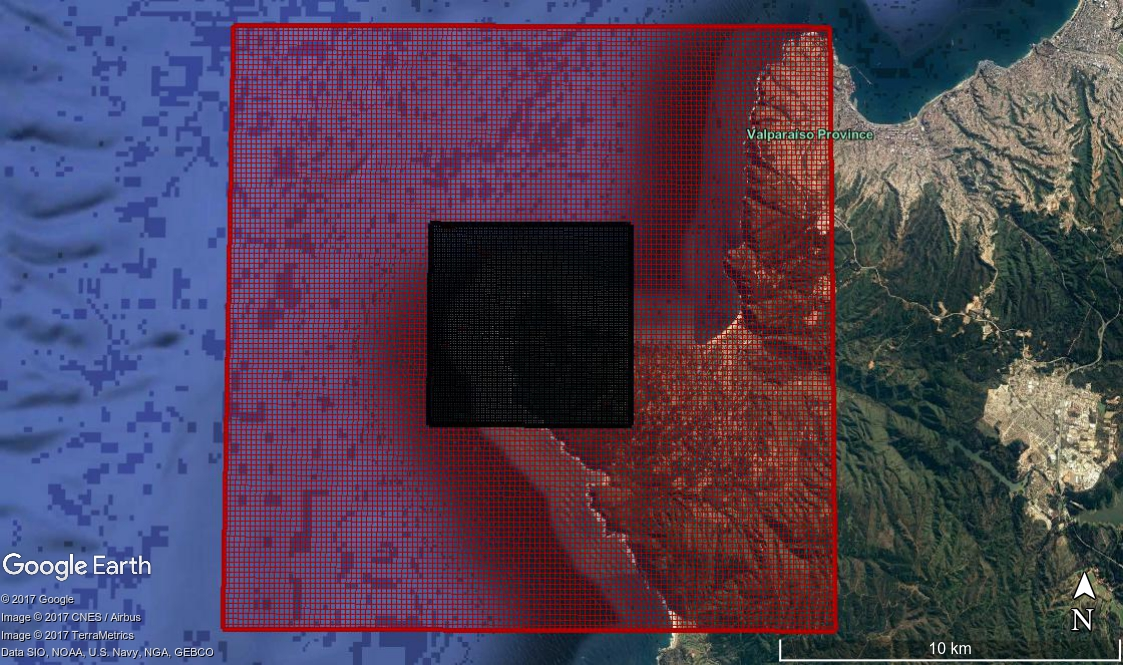
\includegraphics[width=0.95\linewidth]{Imagenes/d02d01}
	\caption{Dominios mas finos d05 (LES) y d06 (LES).}
	\label{fig:0506}
\end{figure}
Cada malla consta de $121\times 121$ nodos en el sentido horizontal y 47 nodos en sentido vertical. Existe un refinamiento de la malla en la cercanía a la superficie de modo de tener los 10 primeros niveles dentro de los primeros 300 [m] de atmósfera.

Debido a la naturaleza de la coordenada vertical utilizada en el kernel del programa, el $\Delta z$ no es constante en todos los niveles verticales, ni en cada columna. Sin embargo, es posible tener una idea sobre la manera en la que está distribuida la malla al considerar el promedio de altura en la coordenada. Este análisis se puede ver en la figura

\begin{figure}[H]
	\centering
	\includegraphics[width=0.8\linewidth,page=9,trim={1cm 6cm 1cm 7.85cm},clip]{Imagenes/perfil_medio}
	\caption{Distribución malla vertical.}
	\label{fig:vertical_mesh}
\end{figure}
\section{Resolución Temporal}
Para la simulación se utiliza un paso de tiempo físico constante. Para no tener problemas de inestabilidades y que el modelo diverja, se opta por una relación empírica conservadora que es parte de las buenas prácticas en el uso del WRF. Se utiliza:
\begin{equation}
\Delta t \approx \Delta x
\end{equation}
Donde $\Delta x$ tiene unidades de [km]. Luego, el paso de tiempo para el dominio mas grande será $\Delta x=12$ [s] y este valor va reduciéndose 1/3 en cada dominio anidado. Utilizando este valor no se presentaron problemas en el desarrollo de las iteraciones.
\section{Condiciones de Borde}
Para inicializar el modelo y para proveer de información en los contornos cada 6 horas, se utilizan los datos de los análisis operacionales provenientes del modelo global GFS con resolución de $0.5^\circ$ ($\approx 55.6$ [km])

Por otra parte, como el dominio mas grande a simular cae dentro de lo que es una simulación de mesoescala y tomando en consideración las proyecciones debido a la curvatura de la tierra para esta zona en particular, se decide fijar la condición de borde superior para la coordenada vertical de presión a $p_{dht} = 5000$ [kPa] siguiendo la recomendación del manual del programa.
\section{Información del Terreno}
Debido a que los últimos 3 dominios son de 450, 150 y 50 [m] respectivamente en sus tamaños de malla, es necesario proveer al modelo información superficial de alta resolución. Para la topografía se utilizan los datos de la operación satelital SRTM de la NASA que tienen resolución de 3 segundos de arco. Para las propiedades de la superficie como vegetación, rugosidad, tipo de uso de suelo se utilizan los datos que provienen de los instrumentos satelitales MODIS.
\section{Parametrizaciones}
\begin{table}[h!]
	\caption{Esquemas de Parametrización Utilizados.}\label{tab:esquemas}
	\centering
	\begin{tabular}{lllllll}
		\toprule
		Física 					& d01	&	d02	&	d03	&	d04	&	d05	&	d06 \\
		\midrule
		Micro-físicas		 	& WSM5 & WSM5 & WSM5 &WSM5&WSM5&WSM5  \\
		Cúmulos			 		& Grell & -- & -- & -- & -- & -- \\ 
		Capa Superficial	 	& MM5 & MM5 & MM5 & MM5 & MM5 & MM5 \\
		PBL				 		& YSU & YSU & YSU & -- & -- & -- \\
		Modelo de Suelo 		& Dif. & Dif. & Dif. & Dif. & Dif. & Dif. 	\\
		Rad. Onda Larga	& RRTM &RRTM&RRTM&RRTM&RRTM&RRTM \\
		Rad. Onda Corta	& Dudhia &Dudhia&Dudhia&Dudhia&Dudhia&Dudhia \\
		\bottomrule
	\end{tabular}
\end{table}
\section{Monitoreo de Variables}
Además de obtener información acerca del comportamiento del flujo en todo el dominio a simular, se fijan algunos puntos característicos del sitio para extraer información adicional.

En específico se fija:
\begin{itemize*}
	\item (-71.716 ,-33.103) : Obtención de series de tiempo para los primeros 15 niveles verticales.
	\item (-71.708 ,-33.115) Obtención de perfil.
	\item (-71.730 ,-33.110) Obtención de perfil.
	\item (-71.704 ,-33.104) Obtención de perfil.
\end{itemize*}

La ubicación de estos puntos en el mapa se pueden observar en la Figura \ref{fig:monitor} donde con color rojo está el punto designado para la serie de tiempo, y los puntos de perfil están con color negro.
\begin{figure}[H]
	\centering
	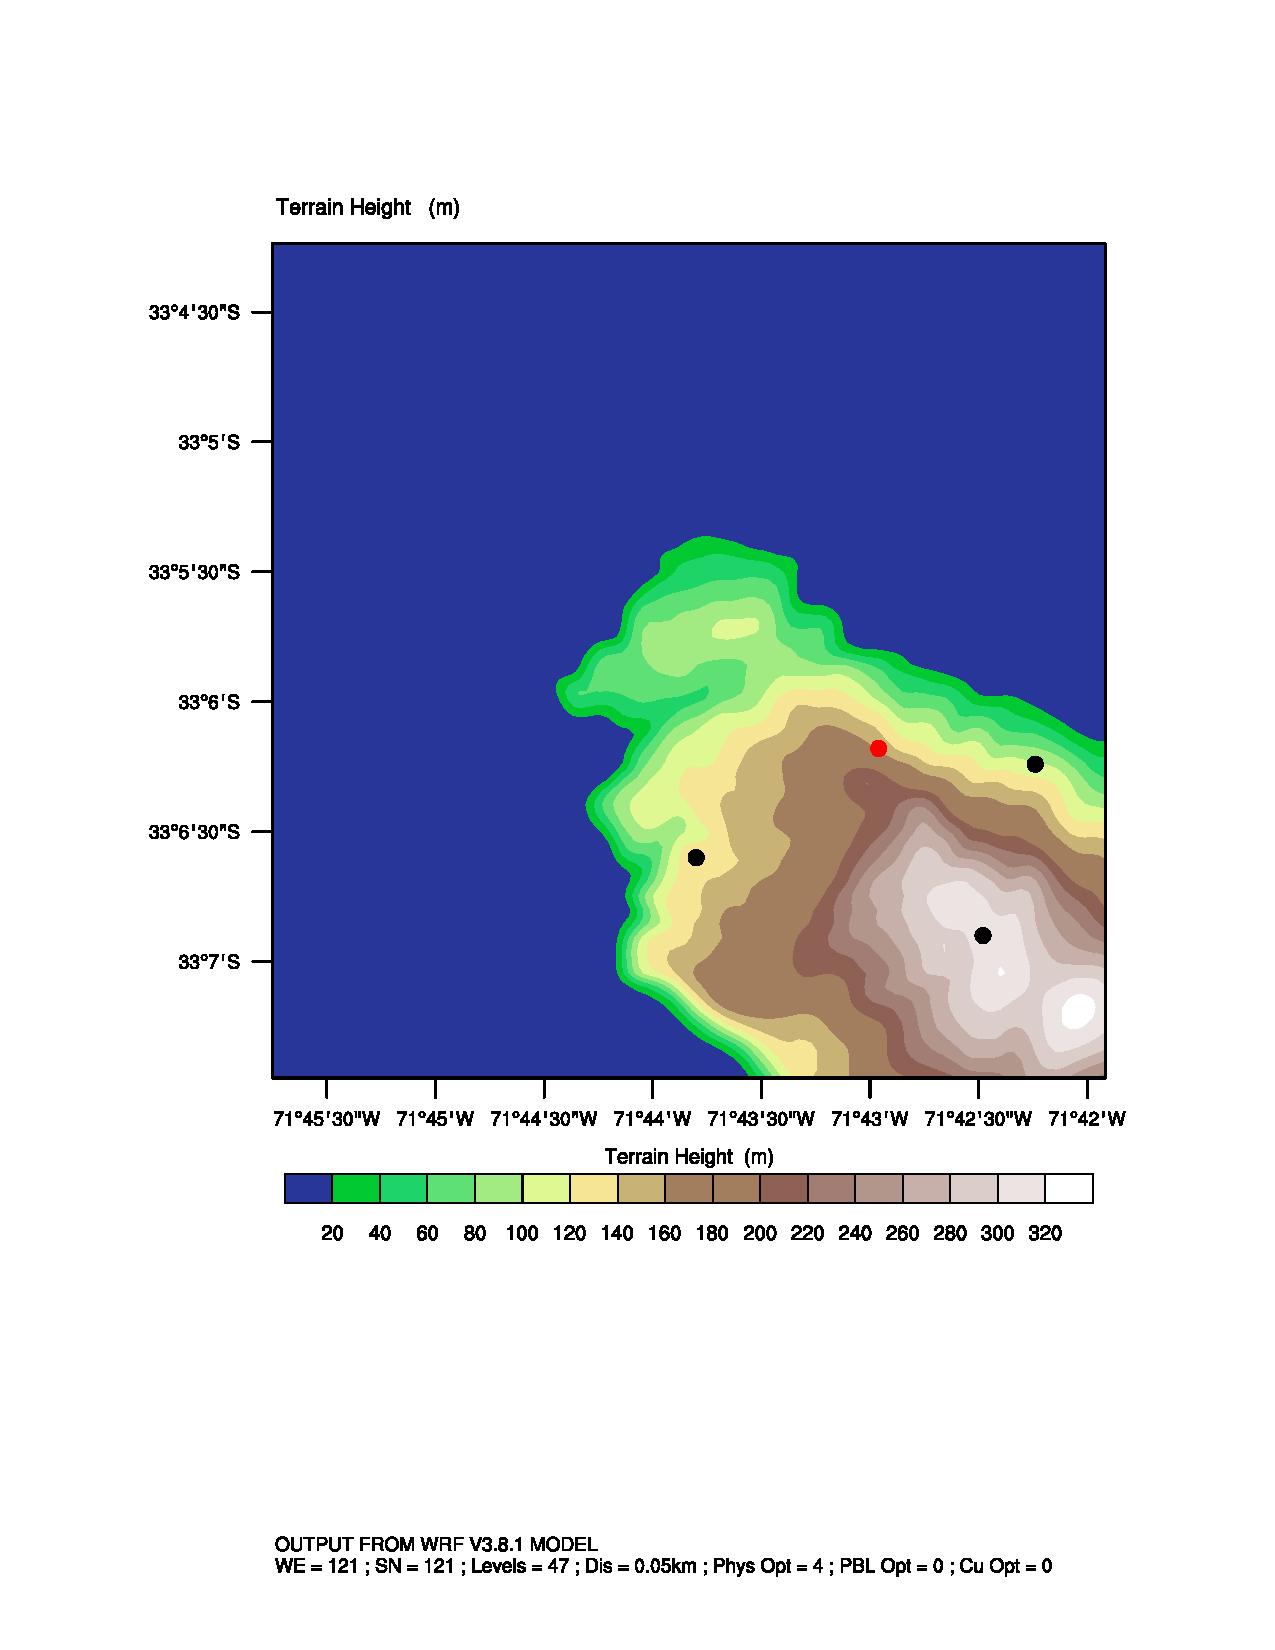
\includegraphics[width=0.85\linewidth,trim={1cm 7cm -1cm 4cm},clip]{Imagenes/altura}
	\caption{Puntos de monitoreo dominio d06.}
	\label{fig:monitor}
\end{figure}